% Options for packages loaded elsewhere
\PassOptionsToPackage{unicode}{hyperref}
\PassOptionsToPackage{hyphens}{url}
%
\documentclass[
]{article}
\usepackage{lmodern}
\usepackage{amssymb,amsmath}
\usepackage{ifxetex,ifluatex}
\ifnum 0\ifxetex 1\fi\ifluatex 1\fi=0 % if pdftex
  \usepackage[T1]{fontenc}
  \usepackage[utf8]{inputenc}
  \usepackage{textcomp} % provide euro and other symbols
\else % if luatex or xetex
  \usepackage{unicode-math}
  \defaultfontfeatures{Scale=MatchLowercase}
  \defaultfontfeatures[\rmfamily]{Ligatures=TeX,Scale=1}
\fi
% Use upquote if available, for straight quotes in verbatim environments
\IfFileExists{upquote.sty}{\usepackage{upquote}}{}
\IfFileExists{microtype.sty}{% use microtype if available
  \usepackage[]{microtype}
  \UseMicrotypeSet[protrusion]{basicmath} % disable protrusion for tt fonts
}{}
\makeatletter
\@ifundefined{KOMAClassName}{% if non-KOMA class
  \IfFileExists{parskip.sty}{%
    \usepackage{parskip}
  }{% else
    \setlength{\parindent}{0pt}
    \setlength{\parskip}{6pt plus 2pt minus 1pt}}
}{% if KOMA class
  \KOMAoptions{parskip=half}}
\makeatother
\usepackage{xcolor}
\IfFileExists{xurl.sty}{\usepackage{xurl}}{} % add URL line breaks if available
\IfFileExists{bookmark.sty}{\usepackage{bookmark}}{\usepackage{hyperref}}
\hypersetup{
  pdftitle={The Linear Model},
  pdfauthor={Livio Finos},
  hidelinks,
  pdfcreator={LaTeX via pandoc}}
\urlstyle{same} % disable monospaced font for URLs
\usepackage[margin=1in]{geometry}
\usepackage{color}
\usepackage{fancyvrb}
\newcommand{\VerbBar}{|}
\newcommand{\VERB}{\Verb[commandchars=\\\{\}]}
\DefineVerbatimEnvironment{Highlighting}{Verbatim}{commandchars=\\\{\}}
% Add ',fontsize=\small' for more characters per line
\usepackage{framed}
\definecolor{shadecolor}{RGB}{248,248,248}
\newenvironment{Shaded}{\begin{snugshade}}{\end{snugshade}}
\newcommand{\AlertTok}[1]{\textcolor[rgb]{0.94,0.16,0.16}{#1}}
\newcommand{\AnnotationTok}[1]{\textcolor[rgb]{0.56,0.35,0.01}{\textbf{\textit{#1}}}}
\newcommand{\AttributeTok}[1]{\textcolor[rgb]{0.77,0.63,0.00}{#1}}
\newcommand{\BaseNTok}[1]{\textcolor[rgb]{0.00,0.00,0.81}{#1}}
\newcommand{\BuiltInTok}[1]{#1}
\newcommand{\CharTok}[1]{\textcolor[rgb]{0.31,0.60,0.02}{#1}}
\newcommand{\CommentTok}[1]{\textcolor[rgb]{0.56,0.35,0.01}{\textit{#1}}}
\newcommand{\CommentVarTok}[1]{\textcolor[rgb]{0.56,0.35,0.01}{\textbf{\textit{#1}}}}
\newcommand{\ConstantTok}[1]{\textcolor[rgb]{0.00,0.00,0.00}{#1}}
\newcommand{\ControlFlowTok}[1]{\textcolor[rgb]{0.13,0.29,0.53}{\textbf{#1}}}
\newcommand{\DataTypeTok}[1]{\textcolor[rgb]{0.13,0.29,0.53}{#1}}
\newcommand{\DecValTok}[1]{\textcolor[rgb]{0.00,0.00,0.81}{#1}}
\newcommand{\DocumentationTok}[1]{\textcolor[rgb]{0.56,0.35,0.01}{\textbf{\textit{#1}}}}
\newcommand{\ErrorTok}[1]{\textcolor[rgb]{0.64,0.00,0.00}{\textbf{#1}}}
\newcommand{\ExtensionTok}[1]{#1}
\newcommand{\FloatTok}[1]{\textcolor[rgb]{0.00,0.00,0.81}{#1}}
\newcommand{\FunctionTok}[1]{\textcolor[rgb]{0.00,0.00,0.00}{#1}}
\newcommand{\ImportTok}[1]{#1}
\newcommand{\InformationTok}[1]{\textcolor[rgb]{0.56,0.35,0.01}{\textbf{\textit{#1}}}}
\newcommand{\KeywordTok}[1]{\textcolor[rgb]{0.13,0.29,0.53}{\textbf{#1}}}
\newcommand{\NormalTok}[1]{#1}
\newcommand{\OperatorTok}[1]{\textcolor[rgb]{0.81,0.36,0.00}{\textbf{#1}}}
\newcommand{\OtherTok}[1]{\textcolor[rgb]{0.56,0.35,0.01}{#1}}
\newcommand{\PreprocessorTok}[1]{\textcolor[rgb]{0.56,0.35,0.01}{\textit{#1}}}
\newcommand{\RegionMarkerTok}[1]{#1}
\newcommand{\SpecialCharTok}[1]{\textcolor[rgb]{0.00,0.00,0.00}{#1}}
\newcommand{\SpecialStringTok}[1]{\textcolor[rgb]{0.31,0.60,0.02}{#1}}
\newcommand{\StringTok}[1]{\textcolor[rgb]{0.31,0.60,0.02}{#1}}
\newcommand{\VariableTok}[1]{\textcolor[rgb]{0.00,0.00,0.00}{#1}}
\newcommand{\VerbatimStringTok}[1]{\textcolor[rgb]{0.31,0.60,0.02}{#1}}
\newcommand{\WarningTok}[1]{\textcolor[rgb]{0.56,0.35,0.01}{\textbf{\textit{#1}}}}
\usepackage{longtable,booktabs}
% Correct order of tables after \paragraph or \subparagraph
\usepackage{etoolbox}
\makeatletter
\patchcmd\longtable{\par}{\if@noskipsec\mbox{}\fi\par}{}{}
\makeatother
% Allow footnotes in longtable head/foot
\IfFileExists{footnotehyper.sty}{\usepackage{footnotehyper}}{\usepackage{footnote}}
\makesavenoteenv{longtable}
\usepackage{graphicx,grffile}
\makeatletter
\def\maxwidth{\ifdim\Gin@nat@width>\linewidth\linewidth\else\Gin@nat@width\fi}
\def\maxheight{\ifdim\Gin@nat@height>\textheight\textheight\else\Gin@nat@height\fi}
\makeatother
% Scale images if necessary, so that they will not overflow the page
% margins by default, and it is still possible to overwrite the defaults
% using explicit options in \includegraphics[width, height, ...]{}
\setkeys{Gin}{width=\maxwidth,height=\maxheight,keepaspectratio}
% Set default figure placement to htbp
\makeatletter
\def\fps@figure{htbp}
\makeatother
\setlength{\emergencystretch}{3em} % prevent overfull lines
\providecommand{\tightlist}{%
  \setlength{\itemsep}{0pt}\setlength{\parskip}{0pt}}
\setcounter{secnumdepth}{5}

\title{The Linear Model}
\author{Livio Finos}
\date{}

\begin{document}
\maketitle

{
\setcounter{tocdepth}{2}
\tableofcontents
}
\hypertarget{outline}{%
\section{Outline}\label{outline}}

\hypertarget{outline-1}{%
\subsection{Outline}\label{outline-1}}

\begin{itemize}
\tightlist
\item
  Covariance and Correlation
\item
  Simple Linear Model
\item
  Analysis of the residuals
\item
  Multiple Linear Model
\item
  2 sample t-test, Anova
\item
  Interaction terms, Ancova
\end{itemize}

\hypertarget{the-age-vs-reaction-time-dataset}{%
\subsection{The Age vs Reaction Time
Dataset}\label{the-age-vs-reaction-time-dataset}}

The reaction time of these subjects was tested by having them grab a
meter stick after it was released by the tester. The number of
centimeters that the meter stick dropped before being caught is a direct
measure of the person's response time.

The values of \texttt{Age} are in years. The \texttt{Gender} is coded as
\texttt{F} for female and \texttt{M} for male. The values of
\texttt{Reaction.Time} are in centimeters.

(data are fictitious)

To read the data

\begin{Shaded}
\begin{Highlighting}[]
\KeywordTok{data}\NormalTok{(reaction,}\DataTypeTok{package =} \StringTok{"flip"}\NormalTok{)}
\CommentTok{# or download it from: https://github.com/livioivil/flip/tree/master/data}
\CommentTok{# or from this folder:}
\CommentTok{# load("./dataset/reaction.rda")}
\CommentTok{# str (reaction)}
\end{Highlighting}
\end{Shaded}

We plot the data

\begin{Shaded}
\begin{Highlighting}[]
\KeywordTok{plot}\NormalTok{(}\DataTypeTok{x=}\NormalTok{reaction}\OperatorTok{$}\NormalTok{Age,}\DataTypeTok{y=}\NormalTok{reaction}\OperatorTok{$}\NormalTok{Reaction.Time,}\DataTypeTok{pch=}\DecValTok{20}\NormalTok{,}\DataTypeTok{col=}\DecValTok{2}\NormalTok{,}\DataTypeTok{cex=}\DecValTok{2}\NormalTok{)}
\end{Highlighting}
\end{Shaded}

\begin{center}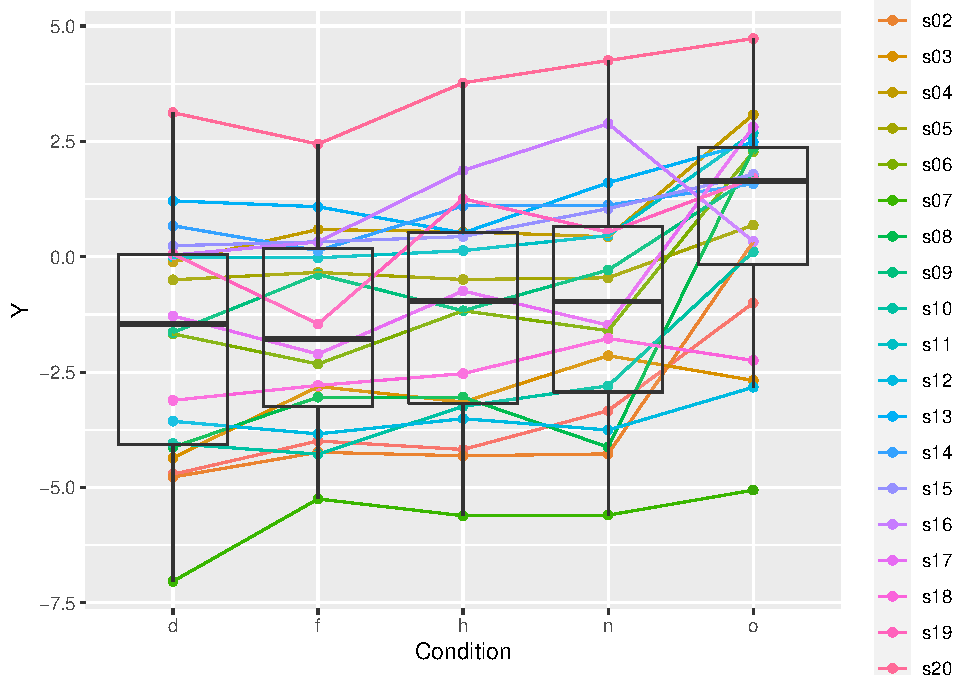
\includegraphics{LinearModel_booklet_files/figure-latex/unnamed-chunk-3-1} \end{center}

\hypertarget{measures-of-dependence-and-the-simple-linear-model}{%
\section{Measures of Dependence and the Simple linear
model}\label{measures-of-dependence-and-the-simple-linear-model}}

\hypertarget{measuring-the-dependence}{%
\subsection{Measuring the dependence}\label{measuring-the-dependence}}

we define:

\begin{itemize}
\tightlist
\item
  \(X=Age\)\\
\item
  \(Y=Reaction.Time\)
\end{itemize}

We review some famous index to measure the (linear) dependence among two
variables

\hypertarget{covariance-and-variance}{%
\subsection{Covariance and Variance}\label{covariance-and-variance}}

\textbf{Covariance} between \(X\) and \(Y\):

\(\sigma_{xy}=\frac{\sum_{i=1} ^ n (x_i- \bar{x}) (y_i- \bar{y} )}{n}\)

\begin{itemize}
\tightlist
\item
  values between \(- \infty\) and \(\infty\)\\
\item
  \(\sigma_{xy} \approx 0\): there is no dependency between \(X\) and
  \(Y\)\\
\item
  \(\sigma_{xy} >> (<<) 0\): there is a strong positive (negative)
  dependency between \(X\) and \(Y\)
\end{itemize}

\textbf{Variance} of \(X\) (= covariance between \(X\) and \(X\)):

\(\sigma_{xx}=\sigma_{x} ^ 2= \frac{\sum_{i=1} ^ n (x_i- \bar{x}) ^ 2}{n}\)

\textbf{Standard Deviation} of \(X\):

\(\sigma_{xx}=\sqrt{\sigma_{xx}}=\sigma_{x}\)

\hypertarget{correlation}{%
\subsection{Correlation}\label{correlation}}

With the Covariance it is difficult to understand when the relationship
between \(X\) and \(Y\) is strong / weak. We note that

\(- \sigma_{x} \sigma_{y} \leq \sigma_{xy} \leq \sigma_{x} \sigma_{y}\)
is quivalent to
\(-1 \leq \frac{\sigma_{xy}}{\sigma_{x} \sigma_{y}} \leq 1\)

\textbf{Correlation} between \(X\) and \(Y\):

\(\rho_{xy}=\frac{\sigma{xy}}{\sigma_{x} \sigma_{y}} = \frac{\sum_{i=1} ^ n (x_i- \bar{x}) (y_i- \bar{y})}{\sqrt{\sum_{i=1} ^ n (x_i- \bar{ x}) ^ 2} \sqrt{\sum_{i=1} ^ n (y_i- \bar{y}) ^ 2}}\)

\begin{itemize}
\tightlist
\item
  values between \(-1\) and \(1\)
\item
  \(\rho_{xy} \approx 0\): there is no dependency between \(X\) and
  \(Y\)
\item
  \(\rho_{xy} \approx 1 (-1)\): there is a strong positive (negative)
  dependency between \(X\) and \(Y\)
\end{itemize}

\hypertarget{the-linear-model}{%
\section{The linear model}\label{the-linear-model}}

\hypertarget{linear-trend-the-least-squares-method}{%
\subsection{Linear Trend, the least squares
method}\label{linear-trend-the-least-squares-method}}

We describe the relationship between\\
\texttt{Reaction.Time} and \texttt{Age} with a straight line.

\(Reaction.Time \approx \beta_0 + \beta_1 Age\)\\
\(Y=\beta_0 + \beta_1X\)

Let's draw a line `in the middle' of the data.

The \textbf{least-squares estimator}

We look for the one that passes more `in the middle', the one that
minimizes the sum of the squares of the residues:

\(\hat{\beta}_0\) and \(\hat{\beta}_1\) such that\\
\(\sum_{i=1} ^ n (y_i - (\hat{\beta}_0 + \hat{\beta}_1x_i )) ^ 2\) is
minimum.

Estimates:

\begin{itemize}
\tightlist
\item
  Angular coefficient:
  \(\hat{\beta}_1=\frac{\sigma_{xy}}{\sigma_{xx}}=\rho_{xy}\frac{\sigma_{y}}{\sigma_{x}}=\frac{\sum_{i=1}^n(x_i- \bar{x})(y_i-\bar{y})}{\sum_{i=1}^n (x_i-\bar{x})^2}=\)
  0.2064719\\
\item
  Intercept: \(\hat{\beta}_0=\bar{y}-\hat{\beta}_1\bar{x}=\) 10.3013483
\item
  Response (estimated \(y\)):
  \(\hat{y}_i=\hat{\beta}_0 + \hat{\beta}_1x_i\)
\item
  Residuals (from the estimated response):
  \(y_i - (\hat{\beta}_0 + \hat{\beta}_1 x_i)=y_i- \hat{y}_i\)
\end{itemize}

and therefore the least squares are the sum of the squared residuals:
\(\sum_{i=1} ^ n (y_i- \hat{\beta}_0 - \hat{\beta}_1x_i) ^ 2=\sum_{i=1} ^ n (y_i- \hat{y}_i ) ^ 2\)

A graphical representation:

\begin{Shaded}
\begin{Highlighting}[]
\NormalTok{model=}\KeywordTok{lm}\NormalTok{(Reaction.Time}\OperatorTok{~}\NormalTok{Age,}\DataTypeTok{data=}\NormalTok{reaction)}
\KeywordTok{coefficients}\NormalTok{(model)}
\end{Highlighting}
\end{Shaded}

\begin{verbatim}
## (Intercept)         Age 
##  10.3013483   0.2064719
\end{verbatim}

\begin{Shaded}
\begin{Highlighting}[]
\KeywordTok{plot}\NormalTok{(reaction}\OperatorTok{$}\NormalTok{Age,reaction}\OperatorTok{$}\NormalTok{Reaction.Time,}\DataTypeTok{pch=}\DecValTok{20}\NormalTok{,}\DataTypeTok{col=}\DecValTok{2}\NormalTok{,}\DataTypeTok{cex=}\DecValTok{1}\NormalTok{)}
\NormalTok{coeff=}\KeywordTok{round}\NormalTok{(}\KeywordTok{coefficients}\NormalTok{(model),}\DecValTok{1}\NormalTok{)}
\KeywordTok{title}\NormalTok{(}\KeywordTok{paste}\NormalTok{(}\StringTok{"Y="}\NormalTok{,coeff[}\DecValTok{1}\NormalTok{],}\StringTok{"+"}\NormalTok{,coeff[}\DecValTok{2}\NormalTok{],}\StringTok{"*X"}\NormalTok{))}
\KeywordTok{abline}\NormalTok{(model,}\DataTypeTok{col=}\DecValTok{1}\NormalTok{)}
\end{Highlighting}
\end{Shaded}

\begin{center}\includegraphics{LinearModel_booklet_files/figure-latex/unnamed-chunk-6-1} \end{center}

\hypertarget{interpretation-of-the-coefficients}{%
\subsubsection{Interpretation of the
coefficients}\label{interpretation-of-the-coefficients}}

\begin{itemize}
\tightlist
\item
  \(\beta_0\) indicates the value of \(y\) when \(x=0\) (where the line
  intersects the ordinate axis).
\item
  \(\beta_1\) indicates how much \(y\) grows as a unit of \(x\) grows

  \begin{itemize}
  \tightlist
  \item
    If \(\beta_1=0\) there is no relation between \(x\) and
    \(y\).\(Y\)is constant (horizontal ), knowing\(x\)does not change
    the estimate of \(y\)
  \item
    If \(\beta_1> (<) 0\) the relation between \(x\) and \(y\) is
    positive (negative). When \(X\) passes from \(x\) a \(x + 1\) the
    estimate of \(Y\) changes from \(\hat{y}\) to
    \(\hat{y} + \hat{\beta}_1\)
  \end{itemize}
\end{itemize}

\hypertarget{the-normal-simple-linear-model}{%
\subsection{The normal (simple) linear
model}\label{the-normal-simple-linear-model}}

We assume that the observed values are distributed around true values
\(\beta_0 + \beta_1 X\) according to a Gaussian law:

\(Y=\textrm{linear part} + \textrm{normal error}\)

\(Y=\beta_0 + \beta_1 X + \varepsilon\)

\textbf{Assumptions of the linear model}

\begin{itemize}
\tightlist
\item
  the \(\boldsymbol{y_i=\beta_0 + \beta_1 x_i + \varepsilon_i}\) the
  relationship between \(X\) and the true (mean) \(Y\) is linear.
\item
  the \textbf{observations} are \textbf{independent} each others (
  knowing the value of the \(y_i\)observation does not help me to
  predict the value of \(y_{i + 1}\)). The random part is
  \(\varepsilon_i\), these are the independent terms.
\item
  \(\boldsymbol{\varepsilon_i \sim N (0, \sigma ^ 2), \ \forall i=1, \ldots, n}\)
  errors have normal distribution with zero mean and common variance
  (homoschedasticity: same variance).
\end{itemize}

Let's go back to our data (and model):

\begin{Shaded}
\begin{Highlighting}[]
\KeywordTok{plot}\NormalTok{ (reaction}\OperatorTok{$}\NormalTok{Age, reaction}\OperatorTok{$}\NormalTok{Reaction.Time, }\DataTypeTok{pch =} \DecValTok{20}\NormalTok{, }\DataTypeTok{col =} \DecValTok{1}\NormalTok{, }\DataTypeTok{cex =} \DecValTok{2}\NormalTok{)}
\end{Highlighting}
\end{Shaded}

\begin{center}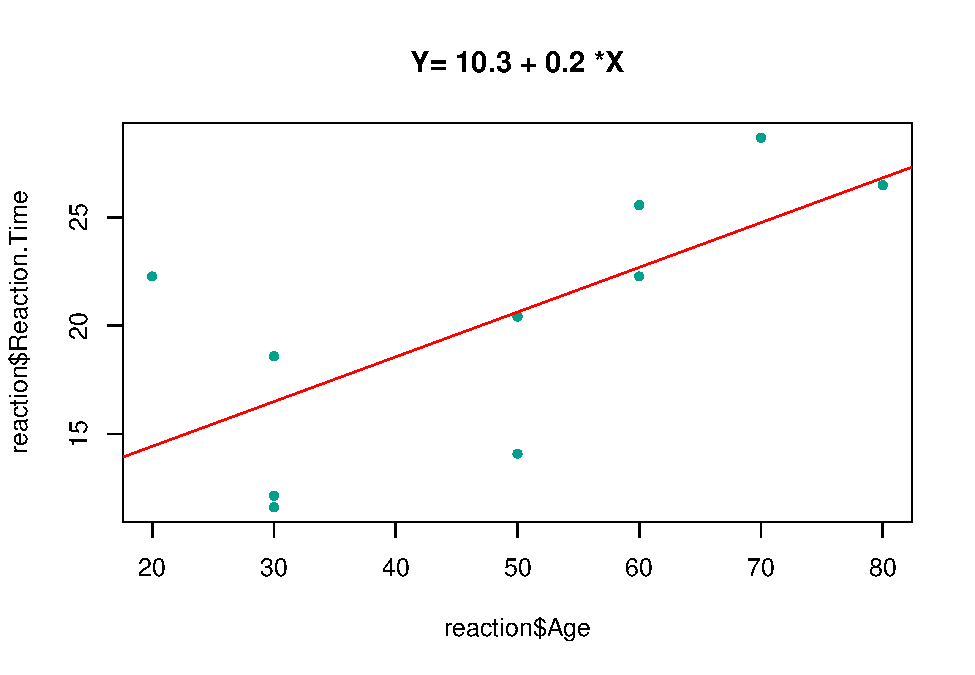
\includegraphics{LinearModel_booklet_files/figure-latex/unnamed-chunk-7-1} \end{center}

\begin{Shaded}
\begin{Highlighting}[]
\CommentTok{# to identify observations on the graph with the mouse}
\CommentTok{# identify (reaction$Age, reaction$Reaction.Time)}
\end{Highlighting}
\end{Shaded}

\hypertarget{fit-the-model-i.e.-estimate-the-parameters}{%
\subsubsection{Fit the model (i.e.~Estimate the
parameters)}\label{fit-the-model-i.e.-estimate-the-parameters}}

\begin{Shaded}
\begin{Highlighting}[]
\NormalTok{model =}\StringTok{ }\KeywordTok{lm}\NormalTok{ (Reaction.Time }\OperatorTok{~}\StringTok{ }\NormalTok{Age, }\DataTypeTok{data =}\NormalTok{ reaction)}
\KeywordTok{summary}\NormalTok{ (model)}
\end{Highlighting}
\end{Shaded}

\begin{verbatim}
## 
## Call:
## lm(formula = Reaction.Time ~ Age, data = reaction)
## 
## Residuals:
##    Min     1Q Median     3Q    Max 
## -6.535 -3.364 -0.272  2.676  7.839 
## 
## Coefficients:
##             Estimate Std. Error t value Pr(>|t|)  
## (Intercept) 10.30135    4.04407   2.547   0.0343 *
## Age          0.20647    0.07841   2.633   0.0300 *
## ---
## Signif. codes:  0 '***' 0.001 '**' 0.01 '*' 0.05 '.' 0.1 ' ' 1
## 
## Residual standard error: 4.678 on 8 degrees of freedom
## Multiple R-squared:  0.4643, Adjusted R-squared:  0.3973 
## F-statistic: 6.934 on 1 and 8 DF,  p-value: 0.03003
\end{verbatim}

(for now) Note that the test\(F\)has the same significance as the t
test.

\hypertarget{graphical-representation-of-the-effect-of-the-age}{%
\subsubsection{Graphical representation of the effect of the
Age}\label{graphical-representation-of-the-effect-of-the-age}}

\begin{Shaded}
\begin{Highlighting}[]
\KeywordTok{library}\NormalTok{ (effects) }\CommentTok{# see:? effect}
\end{Highlighting}
\end{Shaded}

\begin{verbatim}
## Warning: package 'effects' was built under R version 3.6.3
\end{verbatim}

\begin{verbatim}
## Loading required package: carData
\end{verbatim}

\begin{verbatim}
## Warning: package 'carData' was built under R version 3.6.3
\end{verbatim}

\begin{verbatim}
## lattice theme set by effectsTheme()
## See ?effectsTheme for details.
\end{verbatim}

\begin{Shaded}
\begin{Highlighting}[]
\NormalTok{eff <-}\StringTok{ }\KeywordTok{allEffects}\NormalTok{ (model)}
\KeywordTok{plot}\NormalTok{ (eff, }\StringTok{'Age'}\NormalTok{, }\DataTypeTok{ask =}\NormalTok{ F, }\DataTypeTok{main =} \StringTok{''}\NormalTok{)}
\end{Highlighting}
\end{Shaded}

\begin{center}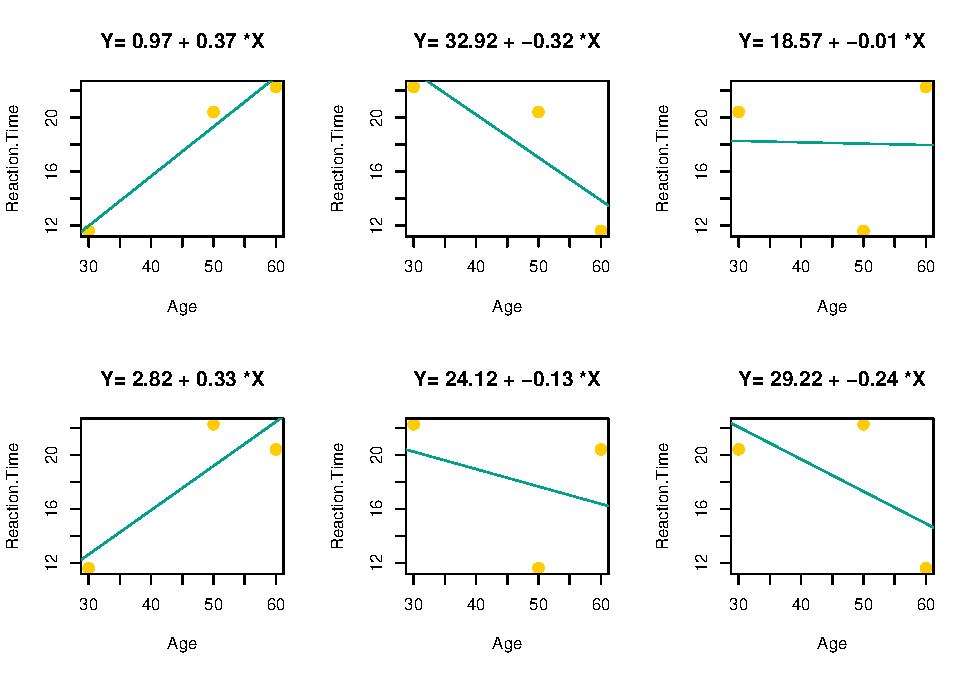
\includegraphics{LinearModel_booklet_files/figure-latex/unnamed-chunk-9-1} \end{center}

\hypertarget{hypothesis-testing}{%
\subsubsection{Hypothesis testing}\label{hypothesis-testing}}

If these assumptions are true,

\(\hat{\beta_1} \sim N (\beta_1, \sigma ^ 2 / \sum (x_i- \bar{x}) ^ 2)\)

We calculate the test statistic:

\(t=\frac{\hat{\beta_1}}{std.dev\ \hat{\beta_1}}=\frac{\hat{\beta_1}}{\sqrt{\sum_{i=1} ^ n (y_i- \hat{y}_i) ^ 2 / \sum (x_i- \bar{x}) ^ 2 / (n-2)}}\)

If \(H_0: \beta_1=0\), \(t \sim t (n-2)\) is true

On \texttt{reaction} data and \(H_1: \beta_1 \neq 0\) (bilateral
alternative)

\begin{Shaded}
\begin{Highlighting}[]
\KeywordTok{summary}\NormalTok{ (model)}
\end{Highlighting}
\end{Shaded}

\begin{verbatim}
## 
## Call:
## lm(formula = Reaction.Time ~ Age, data = reaction)
## 
## Residuals:
##    Min     1Q Median     3Q    Max 
## -6.535 -3.364 -0.272  2.676  7.839 
## 
## Coefficients:
##             Estimate Std. Error t value Pr(>|t|)  
## (Intercept) 10.30135    4.04407   2.547   0.0343 *
## Age          0.20647    0.07841   2.633   0.0300 *
## ---
## Signif. codes:  0 '***' 0.001 '**' 0.01 '*' 0.05 '.' 0.1 ' ' 1
## 
## Residual standard error: 4.678 on 8 degrees of freedom
## Multiple R-squared:  0.4643, Adjusted R-squared:  0.3973 
## F-statistic: 6.934 on 1 and 8 DF,  p-value: 0.03003
\end{verbatim}

\hypertarget{the-multiple-linear-model}{%
\subsection{The Multiple Linear model}\label{the-multiple-linear-model}}

The simple linear model is `easily' extensible to the Multiple Linear
Model. Formally we have the same elements, we only expect the linear
combination of multiple variables.

\(Y = \textrm {linear part} + \textrm {normal error}\)

\(Y = \beta_0 + \beta_1 X_1 + \ldots + \beta_p X_p + \varepsilon\)

Thus we describe a (hyper) plan of size \(p\).

\textbf{Assumptions of Multiple linear model}

They are the same as the simple linear model

\begin{itemize}
\item
  \begin{enumerate}
  \def\labelenumi{\roman{enumi})}
  \tightlist
  \item
    \(y_i = \beta_0 + \beta_1 x_{1i} + \ldots + \beta_p x_{pi} + \varepsilon_i\)
    the relationship between X and Y is truly linear, less than the
    error term\(\varepsilon_i\)
  \end{enumerate}
\item
  \begin{enumerate}
  \def\labelenumi{\roman{enumi})}
  \setcounter{enumi}{1}
  \tightlist
  \item
    the \textbf{observations} are among them \textbf{independent}
  \end{enumerate}
\item
  \begin{enumerate}
  \def\labelenumi{\roman{enumi})}
  \setcounter{enumi}{2}
  \tightlist
  \item
    \(\boldsymbol {\varepsilon_i \sim N (0, \sigma ^2), \ \forall i = 1, \ldots, n}\)
  \end{enumerate}
\end{itemize}

(we will return to the multiple model later)

\hypertarget{linear-regression-in-r}{%
\subsection{Linear regression in R}\label{linear-regression-in-r}}

\texttt{\textgreater{}\ lm\ (formula,\ ...)}

where: \texttt{formula} specifies the link between the employee and the
independent (or predictors)

\hypertarget{examples-of-regression-model-specification}{%
\subsubsection{Examples of regression model
specification}\label{examples-of-regression-model-specification}}

Let \(y\) be the dependent variable and \(x\) and \(z\) two predictors

\begin{longtable}[]{@{}ll@{}}
\toprule
\begin{minipage}[b]{0.41\columnwidth}\raggedright
\textbf{Regression}\strut
\end{minipage} & \begin{minipage}[b]{0.53\columnwidth}\raggedright
\textbf{Regression in R}\strut
\end{minipage}\tabularnewline
\midrule
\endhead
\begin{minipage}[t]{0.41\columnwidth}\raggedright
\(y = \beta_{0} + \beta_{1} x + \varepsilon\)\strut
\end{minipage} & \begin{minipage}[t]{0.53\columnwidth}\raggedright
\(lm (y \sim x)\)\strut
\end{minipage}\tabularnewline
\begin{minipage}[t]{0.41\columnwidth}\raggedright
\(y = \beta_{0} + \beta_{1} x + \beta_{2} z + \varepsilon\)\strut
\end{minipage} & \begin{minipage}[t]{0.53\columnwidth}\raggedright
\(lm (y \sim x + z)\)\strut
\end{minipage}\tabularnewline
\begin{minipage}[t]{0.41\columnwidth}\raggedright
\(y = \beta_{0} + \beta_{1} x + \beta_{2} z + \beta_{3} xz + \varepsilon\)\strut
\end{minipage} & \begin{minipage}[t]{0.53\columnwidth}\raggedright
\(lm (y \sim x + z + x: z)\)\strut
\end{minipage}\tabularnewline
\begin{minipage}[t]{0.41\columnwidth}\raggedright
\(y = \beta_{0} + \beta_{1} x + \beta_{2} z + \beta_{3} xz + \varepsilon\)\strut
\end{minipage} & \begin{minipage}[t]{0.53\columnwidth}\raggedright
\(lm (y \sim x * z)\)\strut
\end{minipage}\tabularnewline
\bottomrule
\end{longtable}

For other options on specifying an R model, see:
\texttt{\textgreater{}?\ formula}

\hypertarget{basic-steps-of-a-regression-model}{%
\subsubsection{Basic steps of a regression
model}\label{basic-steps-of-a-regression-model}}

\begin{longtable}[]{@{}lll@{}}
\toprule
\textbf{Step} & \textbf{Code R} & \textbf{Libraries}\tabularnewline
\midrule
\endhead
Model construction & \(model = lm(formula)\) & stats\tabularnewline
Check recruitment & \(plot(model)\) & stats\tabularnewline
Evaluation of parameters & \(summary (model)\) & stats\tabularnewline
Analysis of variance & \(anova(model)\) & stats\tabularnewline
Analysis of variance & \(Anova(model, type = `` III '')\) &
car\tabularnewline
Viewing effects & see \(? effect\) & effects\tabularnewline
Comparison with other models * & \(anova (model, model2)\) &
stats\tabularnewline
Comparison with other models * * & \(AIC (model)\);\(AIC (model2)\) &
stats\tabularnewline
\bottomrule
\end{longtable}

* comparison between \emph{nested} models based on the\(F\)test\\
* * model comparison based on the Akaike Information Criterion (AIC) or
on the Bayesian Information Criterion (BIC): see also \textbf{? AIC }

\hypertarget{evaluating-the-validity-of-the-assumptions-the-residuals-of-the-fitted-model}{%
\subsection{Evaluating the validity of the assumptions: the residuals of
the fitted
model}\label{evaluating-the-validity-of-the-assumptions-the-residuals-of-the-fitted-model}}

\begin{Shaded}
\begin{Highlighting}[]
\KeywordTok{par}\NormalTok{ (}\DataTypeTok{mar =} \KeywordTok{c}\NormalTok{ (}\DecValTok{6}\NormalTok{, }\DecValTok{5}\NormalTok{, }\DecValTok{4}\NormalTok{, }\DecValTok{2}\NormalTok{) }\OperatorTok{+}\StringTok{ }\FloatTok{0.1}\NormalTok{)}
\KeywordTok{par}\NormalTok{ (}\DataTypeTok{mfrow =} \KeywordTok{c}\NormalTok{ (}\DecValTok{2}\NormalTok{,}\DecValTok{2}\NormalTok{))}
\KeywordTok{plot}\NormalTok{ (model) }\CommentTok{# see also:? plot.lm for bibliographical references}
\end{Highlighting}
\end{Shaded}

\begin{center}\includegraphics{LinearModel_booklet_files/figure-latex/unnamed-chunk-11-1} \end{center}

\begin{itemize}
\tightlist
\item
  Residual independence?
\item
  Residual conditions?
\item
  Homogeneity variance residues?
\item
  Presence of influential cases?
\end{itemize}

Please, no test of normality, homoschedasticity etc. (check the error of
the first type on the contrary to what you would like).

\hypertarget{supplement-looking-for-influential-cases}{%
\subsubsection{Supplement: Looking for influential
cases}\label{supplement-looking-for-influential-cases}}

\begin{itemize}
\tightlist
\item
  In a statistical model an \emph{influential case} is a statistical
  unit whose observations are strong impact on model parameter estimates
\item
  In regression models, a particularly effective way to identify
  influential values is to use \emph{Cook's distance (Cook, 1977)}
\item
  Given a statistical unit, Cook's distance is a measure of how much the
  regression coefficients of the estimated model would change if this
  unit was omitted
\item
  Greater is Cook's distance, the more the statistical unit helps to
  determine the parameters of the regression model
\end{itemize}

Identification of influential cases:

\begin{itemize}
\tightlist
\item
  In the graph just seen R signals the statistical units with Cook
  distance values close to 0.5 and to 1, values to be considered as
  attention thresholds.
\item
  Fox, 2010, proposes a cut-off for Cook's distance that takes into
  account the number of observations (\(n\)) and the number of
  parameters (\(k\)) of the model: \(\dfrac{4}{(n-k-1)}\)
\end{itemize}

In our case:

\begin{Shaded}
\begin{Highlighting}[]
\CommentTok{# calculation and representation of Cook's distance}
\NormalTok{distances.cook =}\StringTok{ }\KeywordTok{cooks.distance}\NormalTok{ (model)}
\KeywordTok{plot}\NormalTok{ (distances.cook, }\DataTypeTok{xlab =} \StringTok{"observation number"}\NormalTok{, }\DataTypeTok{ylab =} \StringTok{"distance of Cook"}\NormalTok{, }\DataTypeTok{cex =} \FloatTok{1.5}\NormalTok{, }\DataTypeTok{cex.axis =} \FloatTok{1.3}\NormalTok{, }\DataTypeTok{cex.lab =} \FloatTok{1.5}\NormalTok{)}
\CommentTok{# representation of the cutoff line at the value 4 / (n-k-1)}
\NormalTok{n =}\StringTok{ }\KeywordTok{nrow}\NormalTok{ (reaction); k =}\StringTok{ }\KeywordTok{length}\NormalTok{ (}\KeywordTok{coefficients}\NormalTok{ (model))}
\NormalTok{cutoff =}\StringTok{ }\DecValTok{4} \OperatorTok{/}\StringTok{ }\NormalTok{(n}\OperatorTok{-}\NormalTok{k}\DecValTok{-1}\NormalTok{)}
\KeywordTok{abline}\NormalTok{ (}\DataTypeTok{h=}\NormalTok{ cutoff, }\DataTypeTok{lty =} \DecValTok{2}\NormalTok{)}
\KeywordTok{text}\NormalTok{ (}\DecValTok{3}\NormalTok{, cutoff }\OperatorTok{*}\StringTok{ }\FloatTok{.9}\NormalTok{, }\StringTok{"cutoff"}\NormalTok{, }\DataTypeTok{cex =} \FloatTok{1.4}\NormalTok{)}
\end{Highlighting}
\end{Shaded}

\begin{center}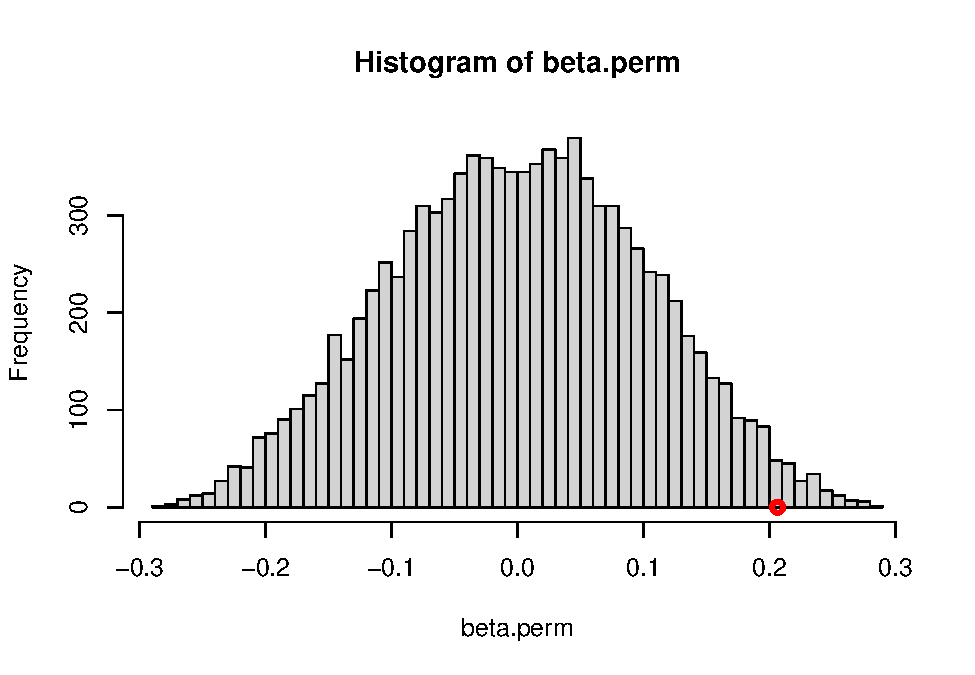
\includegraphics{LinearModel_booklet_files/figure-latex/unnamed-chunk-12-1} \end{center}

\textbf{Remarks}

\begin{itemize}
\tightlist
\item
  Cook's distance is not the only useful indicator for evaluating
  influential cases. For an overview see R:? Influence.measures
\item
  The identification, evaluation and interpretation of influential cases
  are fundamental phases of statistical modeling.
\item
  However these aspects are often underestimated in concrete case
  applications :-(
\end{itemize}

\textbf{Exercise 1.} Build a regression model by eliminating observation
10. How does the model change?

\hypertarget{some-special-cases-t-test-and-anova-etc}{%
\section{Some special cases (t-test and ANOVA
etc)}\label{some-special-cases-t-test-and-anova-etc}}

\hypertarget{the-two-independent-samples-problem}{%
\subsection{The Two-independent-samples
problem}\label{the-two-independent-samples-problem}}

\begin{Shaded}
\begin{Highlighting}[]
\KeywordTok{plot}\NormalTok{ (Reaction.Time }\OperatorTok{~}\StringTok{ }\NormalTok{Gender, }\DataTypeTok{data =}\NormalTok{ reaction, }\DataTypeTok{col =} \DecValTok{2}\OperatorTok{:}\DecValTok{3}\NormalTok{)}
\end{Highlighting}
\end{Shaded}

\begin{center}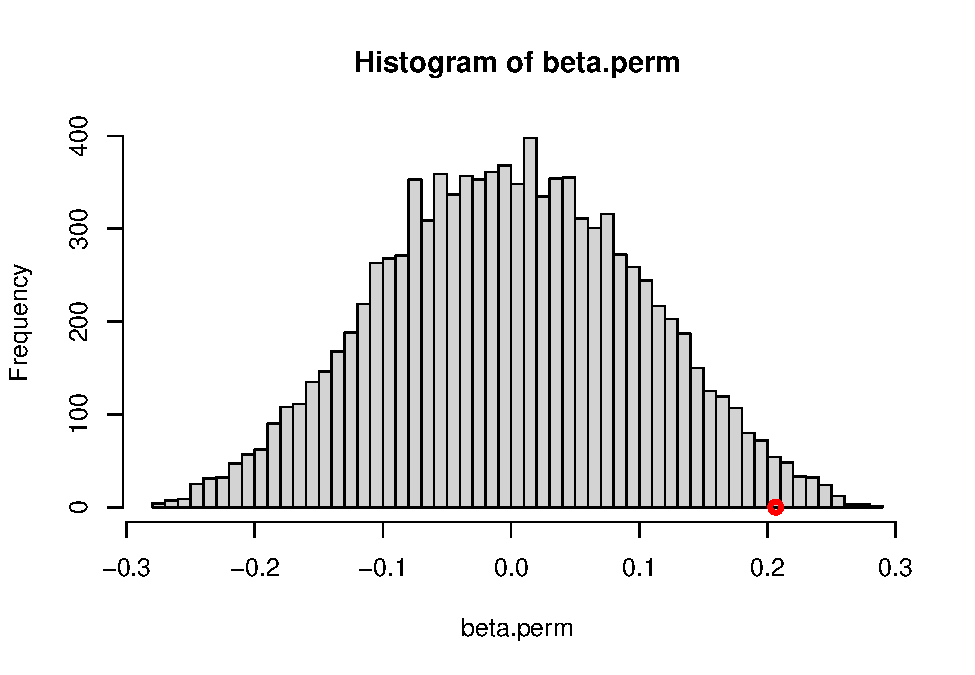
\includegraphics{LinearModel_booklet_files/figure-latex/unnamed-chunk-13-1} \end{center}

Is it possible to estimate a model that uses \texttt{Gender} as a
predictor? How?

Use \texttt{Gender} as if it where a quantitative variable:

\begin{Shaded}
\begin{Highlighting}[]
\NormalTok{modelGender =}\StringTok{ }\KeywordTok{lm}\NormalTok{ (Reaction.Time }\OperatorTok{~}\StringTok{ }\NormalTok{Gender, }\DataTypeTok{data =}\NormalTok{ reaction)}
\KeywordTok{summary}\NormalTok{ (modelGender)}
\end{Highlighting}
\end{Shaded}

\begin{verbatim}
## 
## Call:
## lm(formula = Reaction.Time ~ Gender, data = reaction)
## 
## Residuals:
##    Min     1Q Median     3Q    Max 
## -4.966 -3.188 -1.568  1.933  9.894 
## 
## Coefficients:
##             Estimate Std. Error t value Pr(>|t|)    
## (Intercept)   23.838      2.210   10.79 4.81e-06 ***
## GenderM       -7.252      3.126   -2.32   0.0489 *  
## ---
## Signif. codes:  0 '***' 0.001 '**' 0.01 '*' 0.05 '.' 0.1 ' ' 1
## 
## Residual standard error: 4.942 on 8 degrees of freedom
## Multiple R-squared:  0.4022, Adjusted R-squared:  0.3275 
## F-statistic: 5.383 on 1 and 8 DF,  p-value: 0.04891
\end{verbatim}

\begin{Shaded}
\begin{Highlighting}[]
\KeywordTok{plot}\NormalTok{ (modelGender)}
\end{Highlighting}
\end{Shaded}

\begin{center}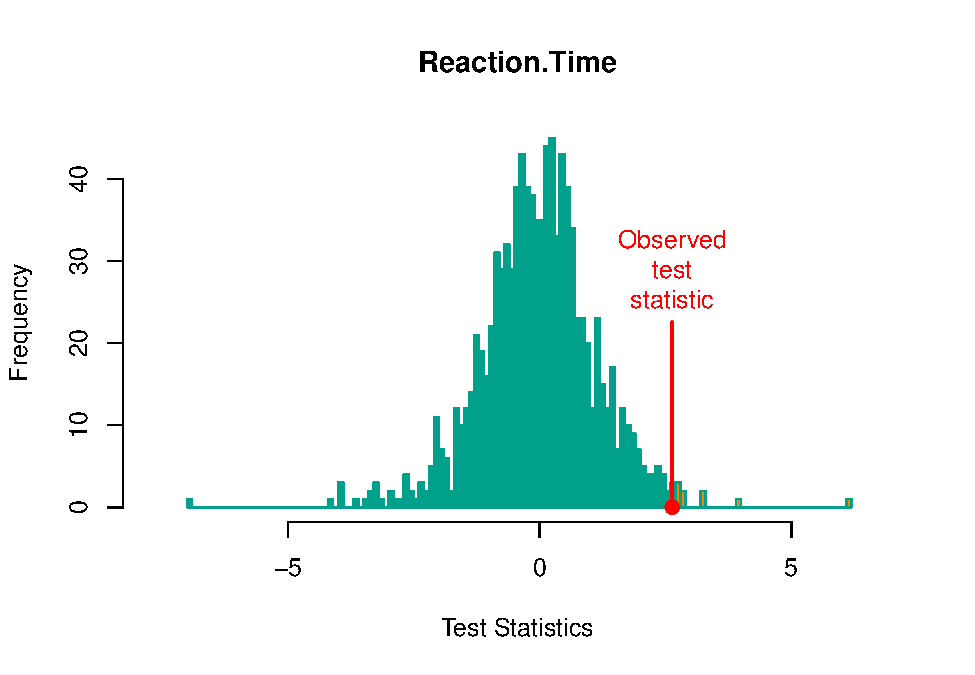
\includegraphics{LinearModel_booklet_files/figure-latex/unnamed-chunk-14-1} \end{center}

\begin{center}\includegraphics{LinearModel_booklet_files/figure-latex/unnamed-chunk-14-2} \end{center}

\begin{center}\includegraphics{LinearModel_booklet_files/figure-latex/unnamed-chunk-14-3} \end{center}

\begin{center}\includegraphics{LinearModel_booklet_files/figure-latex/unnamed-chunk-14-4} \end{center}

. How do we interpret the coefficients? . What kind of model are we
estimating? . What are the differences with my old friend t-test for two
independent samples ??

have a look here:

\begin{Shaded}
\begin{Highlighting}[]
\KeywordTok{model.matrix}\NormalTok{(Reaction.Time }\OperatorTok{~}\StringTok{ }\NormalTok{Gender, }\DataTypeTok{data =}\NormalTok{ reaction)}
\end{Highlighting}
\end{Shaded}

\begin{verbatim}
##    (Intercept) GenderM
## 1            1       0
## 2            1       0
## 3            1       1
## 4            1       0
## 5            1       1
## 6            1       0
## 7            1       1
## 8            1       1
## 9            1       0
## 10           1       1
## attr(,"assign")
## [1] 0 1
## attr(,"contrasts")
## attr(,"contrasts")$Gender
## [1] "contr.treatment"
\end{verbatim}

\begin{Shaded}
\begin{Highlighting}[]
\KeywordTok{by}\NormalTok{ (reaction}\OperatorTok{$}\NormalTok{Reaction.Time, reaction}\OperatorTok{$}\NormalTok{Gender, mean)}
\end{Highlighting}
\end{Shaded}

\begin{verbatim}
## reaction$Gender: F
## [1] 23.838
## ------------------------------------------------------------ 
## reaction$Gender: M
## [1] 16.586
\end{verbatim}

\begin{Shaded}
\begin{Highlighting}[]
\KeywordTok{t.test}\NormalTok{ (Reaction.Time }\OperatorTok{~}\StringTok{ }\NormalTok{Gender, }\DataTypeTok{data =}\NormalTok{ reaction, }\DataTypeTok{var.equal =} \OtherTok{TRUE}\NormalTok{)}
\end{Highlighting}
\end{Shaded}

\begin{verbatim}
## 
##  Two Sample t-test
## 
## data:  Reaction.Time by Gender
## t = 2.3202, df = 8, p-value = 0.04891
## alternative hypothesis: true difference in means is not equal to 0
## 95 percent confidence interval:
##   0.0443075 14.4596925
## sample estimates:
## mean in group F mean in group M 
##          23.838          16.586
\end{verbatim}

REMARK: The t-test is very often ran allowing for the variance of the
two groups to be different (i.e.~Welch correction -- var.equal = TRUE in
\texttt{R}, the default). In this case regression model (which assumes
homoscedasticity, i.e.~equal variance for all observations) is not
exactly equivalent to the t-test -- despite the two are usually very
close each other.

\hypertarget{analysis-of-variance-anova}{%
\subsection{ANalysis Of VAriance
(ANOVA)}\label{analysis-of-variance-anova}}

\begin{Shaded}
\begin{Highlighting}[]
\NormalTok{reaction}\OperatorTok{$}\NormalTok{Age_categ=}\KeywordTok{cut}\NormalTok{(reaction}\OperatorTok{$}\NormalTok{Age,}\KeywordTok{c}\NormalTok{(}\DecValTok{0}\NormalTok{,}\DecValTok{30}\NormalTok{,}\DecValTok{60}\NormalTok{,}\OtherTok{Inf}\NormalTok{))}
\KeywordTok{table}\NormalTok{(reaction}\OperatorTok{$}\NormalTok{Age_categ)}
\end{Highlighting}
\end{Shaded}

\begin{verbatim}
## 
##   (0,30]  (30,60] (60,Inf] 
##        4        4        2
\end{verbatim}

\begin{Shaded}
\begin{Highlighting}[]
\KeywordTok{plot}\NormalTok{ (Reaction.Time }\OperatorTok{~}\StringTok{ }\NormalTok{Age_categ, }\DataTypeTok{data =}\NormalTok{ reaction, }\DataTypeTok{col =} \DecValTok{2}\OperatorTok{:}\DecValTok{4}\NormalTok{)}
\end{Highlighting}
\end{Shaded}

\begin{center}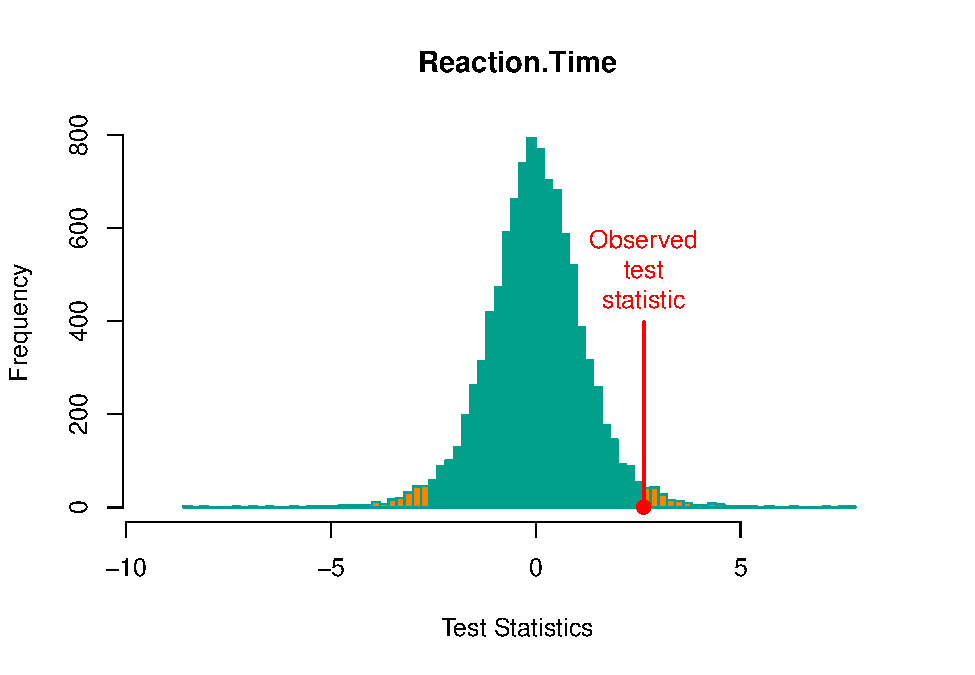
\includegraphics{LinearModel_booklet_files/figure-latex/unnamed-chunk-17-1} \end{center}

Can we use a multiple linear model to fit a categorical variable (with
more than 2 levels)?

Have a look:

\begin{Shaded}
\begin{Highlighting}[]
\KeywordTok{model.matrix}\NormalTok{(Reaction.Time }\OperatorTok{~}\StringTok{ }\NormalTok{Age_categ, }\DataTypeTok{data =}\NormalTok{ reaction)}
\end{Highlighting}
\end{Shaded}

\begin{verbatim}
##    (Intercept) Age_categ(30,60] Age_categ(60,Inf]
## 1            1                0                 1
## 2            1                1                 0
## 3            1                0                 0
## 4            1                1                 0
## 5            1                0                 1
## 6            1                1                 0
## 7            1                0                 0
## 8            1                0                 0
## 9            1                0                 0
## 10           1                1                 0
## attr(,"assign")
## [1] 0 1 1
## attr(,"contrasts")
## attr(,"contrasts")$Age_categ
## [1] "contr.treatment"
\end{verbatim}

\begin{Shaded}
\begin{Highlighting}[]
\NormalTok{mod=}\KeywordTok{lm}\NormalTok{(Reaction.Time }\OperatorTok{~}\StringTok{ }\NormalTok{Age_categ, }\DataTypeTok{data =}\NormalTok{ reaction)}
\KeywordTok{summary}\NormalTok{(mod)}
\end{Highlighting}
\end{Shaded}

\begin{verbatim}
## 
## Call:
## lm(formula = Reaction.Time ~ Age_categ, data = reaction)
## 
## Residuals:
##    Min     1Q Median     3Q    Max 
## -6.495 -3.279  0.465  2.246  6.112 
## 
## Coefficients:
##                   Estimate Std. Error t value Pr(>|t|)    
## (Intercept)         16.157      2.331   6.932 0.000225 ***
## Age_categ(30,60]     4.428      3.296   1.343 0.221144    
## Age_categ(60,Inf]   11.418      4.037   2.828 0.025478 *  
## ---
## Signif. codes:  0 '***' 0.001 '**' 0.01 '*' 0.05 '.' 0.1 ' ' 1
## 
## Residual standard error: 4.662 on 7 degrees of freedom
## Multiple R-squared:  0.5346, Adjusted R-squared:  0.4016 
## F-statistic:  4.02 on 2 and 7 DF,  p-value: 0.06878
\end{verbatim}

See the correspondence between overall significance in multiple linear
model (above) and ANOVA (here below):

\begin{Shaded}
\begin{Highlighting}[]
\NormalTok{car}\OperatorTok{::}\KeywordTok{Anova}\NormalTok{(mod)}
\end{Highlighting}
\end{Shaded}

\begin{verbatim}
## Registered S3 methods overwritten by 'car':
##   method                          from
##   influence.merMod                lme4
##   cooks.distance.influence.merMod lme4
##   dfbeta.influence.merMod         lme4
##   dfbetas.influence.merMod        lme4
\end{verbatim}

\begin{verbatim}
## Anova Table (Type II tests)
## 
## Response: Reaction.Time
##           Sum Sq Df F value  Pr(>F)  
## Age_categ 174.74  2  4.0202 0.06878 .
## Residuals 152.13  7                  
## ---
## Signif. codes:  0 '***' 0.001 '**' 0.01 '*' 0.05 '.' 0.1 ' ' 1
\end{verbatim}

\begin{Shaded}
\begin{Highlighting}[]
\CommentTok{# same result: anova(mod)}
\end{Highlighting}
\end{Shaded}

\hypertarget{interaction-model-ancova-model-selection-etc}{%
\section{Interaction model (ANCOVA), model selection
etc}\label{interaction-model-ancova-model-selection-etc}}

\hypertarget{the-multiple-linear-model-with-interaction}{%
\subsection{The Multiple linear model with
interaction}\label{the-multiple-linear-model-with-interaction}}

\[
Y = {\beta} _{0} + {\beta} _{1} X {1} + \beta_{2} X_{2} + \beta_{3} X_{1} X_{2} + \epsilon
\]

where:

\begin{itemize}
\tightlist
\item
  \(Y\)=\(Reaction.Time\)\\
\item
  \(X_{1}\)=\(Age\)\\
\item
  \(X_{2}\)=\(Gender\)
\end{itemize}

\hypertarget{plot-the-relationship-between-reaction.time-and-age-also-considering-the-gender.}{%
\subsubsection{\texorpdfstring{Plot the relationship between
\(Reaction.Time\) and \(Age\) also considering the
\(Gender\).}{Plot the relationship between Reaction.Time and Age also considering the Gender.}}\label{plot-the-relationship-between-reaction.time-and-age-also-considering-the-gender.}}

\begin{Shaded}
\begin{Highlighting}[]
\KeywordTok{plot}\NormalTok{ (reaction}\OperatorTok{$}\NormalTok{Age, reaction}\OperatorTok{$}\NormalTok{Reaction.Time, }\DataTypeTok{col =}\NormalTok{ (reaction}\OperatorTok{$}\NormalTok{Gender }\OperatorTok{==}\StringTok{ "M"}\NormalTok{) }\OperatorTok{+}\StringTok{ }\DecValTok{1}\NormalTok{, }\DataTypeTok{pch =} \DecValTok{20}\NormalTok{, }\DataTypeTok{cex =} \DecValTok{3}\NormalTok{)}
\KeywordTok{legend}\NormalTok{ ( }\StringTok{"bottomright"}\NormalTok{, }\DataTypeTok{legend =} \KeywordTok{c}\NormalTok{ ( }\StringTok{"M"}\NormalTok{, }\StringTok{"F"}\NormalTok{), }\DataTypeTok{pch =} \DecValTok{20}\NormalTok{, }\DataTypeTok{cex =} \DecValTok{2}\NormalTok{, }\DataTypeTok{col =} \KeywordTok{c}\NormalTok{ (}\DecValTok{2}\NormalTok{,}\DecValTok{1}\NormalTok{), }\DataTypeTok{bty =} \StringTok{"n"}\NormalTok{)}
\end{Highlighting}
\end{Shaded}

\begin{center}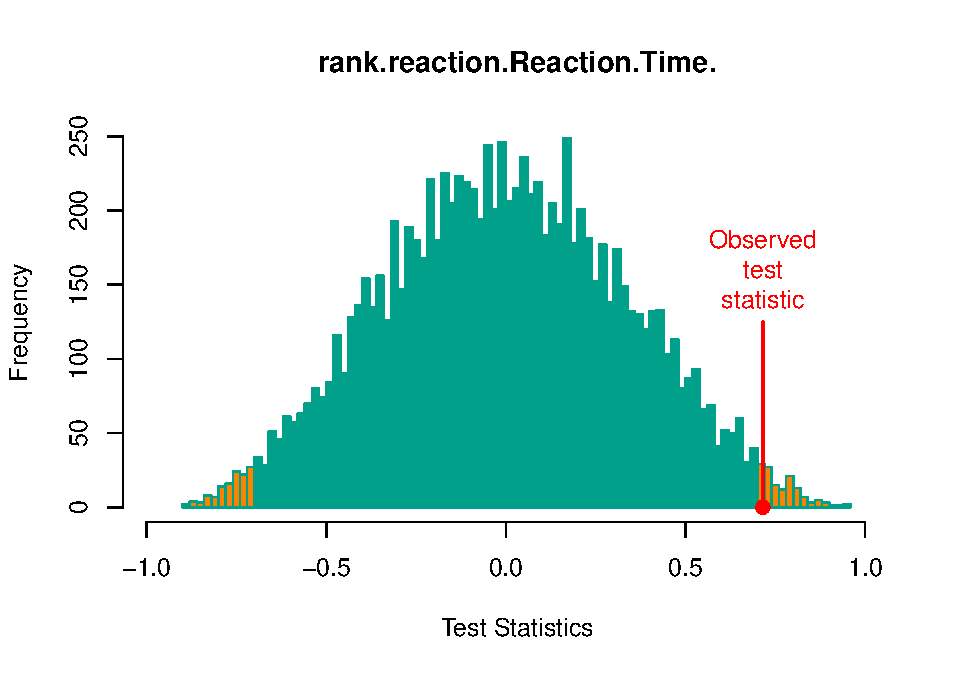
\includegraphics{LinearModel_booklet_files/figure-latex/unnamed-chunk-21-1} \end{center}

We know how to estimate a linear model that includes \(Reaction.Time\)
through the \(Age\). \textbf{EXERCISE:} do it.

How to estimate a model with \(Age\), \(Gender\) and their interaction?

\begin{Shaded}
\begin{Highlighting}[]
\NormalTok{modelFull =}\StringTok{ }\KeywordTok{lm}\NormalTok{ (Reaction.Time }\OperatorTok{~}\StringTok{ }\NormalTok{Age }\OperatorTok{+}\StringTok{ }\NormalTok{Gender }\OperatorTok{+}\StringTok{ }\NormalTok{Age}\OperatorTok{:}\StringTok{ }\NormalTok{Gender, }\DataTypeTok{data =}\NormalTok{ reaction)}
\end{Highlighting}
\end{Shaded}

What predictors (i.e.~independent variables) does R use internally?\\
Have a look:

\begin{Shaded}
\begin{Highlighting}[]
\KeywordTok{model.matrix}\NormalTok{(Reaction.Time }\OperatorTok{~}\StringTok{ }\NormalTok{Age }\OperatorTok{+}\StringTok{ }\NormalTok{Gender }\OperatorTok{+}\StringTok{ }\NormalTok{Age}\OperatorTok{:}\StringTok{ }\NormalTok{Gender, }\DataTypeTok{data =}\NormalTok{ reaction)}
\end{Highlighting}
\end{Shaded}

\begin{verbatim}
##    (Intercept) Age GenderM Age:GenderM
## 1            1  70       0           0
## 2            1  50       0           0
## 3            1  30       1          30
## 4            1  60       0           0
## 5            1  80       1          80
## 6            1  60       0           0
## 7            1  30       1          30
## 8            1  30       1          30
## 9            1  20       0           0
## 10           1  50       1          50
## attr(,"assign")
## [1] 0 1 2 3
## attr(,"contrasts")
## attr(,"contrasts")$Gender
## [1] "contr.treatment"
\end{verbatim}

\textbf{How do we interpret the model?}

\begin{Shaded}
\begin{Highlighting}[]
\KeywordTok{plot}\NormalTok{ (reaction}\OperatorTok{$}\NormalTok{Age, reaction}\OperatorTok{$}\NormalTok{Reaction.Time, }\DataTypeTok{col =}\NormalTok{ (reaction}\OperatorTok{$}\NormalTok{Gender }\OperatorTok{==}\StringTok{ "M"}\NormalTok{) }\OperatorTok{+}\StringTok{ }\DecValTok{1}\NormalTok{, }\DataTypeTok{pch =} \DecValTok{20}\NormalTok{, }\DataTypeTok{cex =} \DecValTok{3}\NormalTok{)}
\KeywordTok{abline}\NormalTok{ (}\KeywordTok{coefficients}\NormalTok{ (modelFull) [}\DecValTok{1}\NormalTok{], }\KeywordTok{coefficients}\NormalTok{ (modelFull) [}\DecValTok{2}\NormalTok{], }\DataTypeTok{col =} \DecValTok{1}\NormalTok{)}
\KeywordTok{abline}\NormalTok{ (}\KeywordTok{coefficients}\NormalTok{ (modelFull) [}\DecValTok{1}\NormalTok{] }\OperatorTok{+}\StringTok{ }\KeywordTok{coefficients}\NormalTok{ (modelFull) [}\DecValTok{3}\NormalTok{], }\KeywordTok{coefficients}\NormalTok{ (modelFull) [}\DecValTok{2}\NormalTok{] }\OperatorTok{+}\StringTok{ }\KeywordTok{coefficients}\NormalTok{ (modelFull) [}\DecValTok{4}\NormalTok{], }\DataTypeTok{col =} \DecValTok{2}\NormalTok{)}
\end{Highlighting}
\end{Shaded}

\begin{center}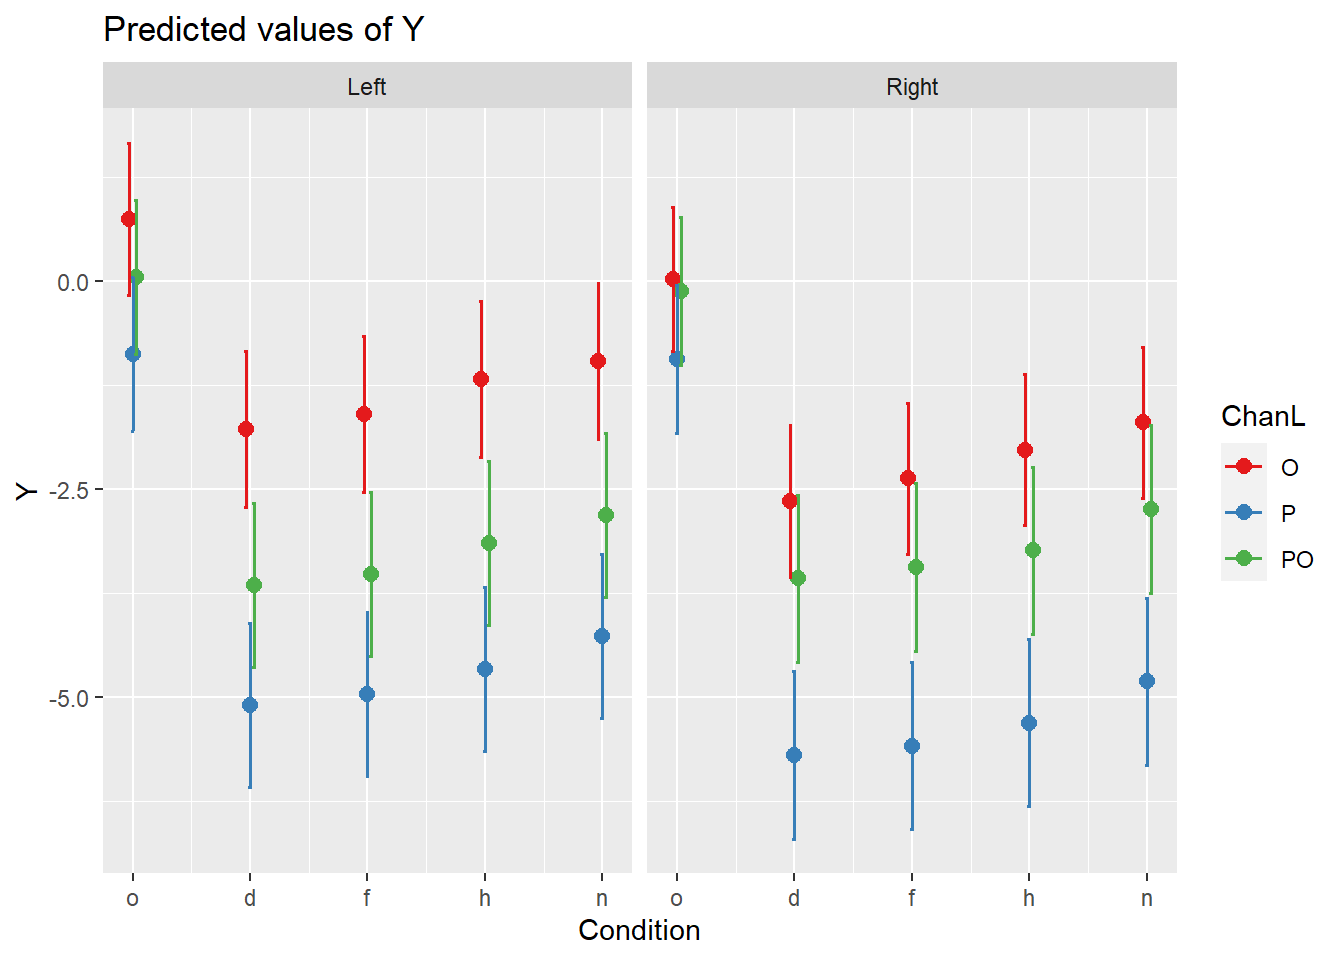
\includegraphics{LinearModel_booklet_files/figure-latex/unnamed-chunk-24-1} \end{center}

\textbf{How do we interpret the results of the analysis?}

\begin{Shaded}
\begin{Highlighting}[]
\KeywordTok{summary}\NormalTok{ (modelFull)}
\end{Highlighting}
\end{Shaded}

\begin{verbatim}
## 
## Call:
## lm(formula = Reaction.Time ~ Age + Gender + Age:Gender, data = reaction)
## 
## Residuals:
##     Min      1Q  Median      3Q     Max 
## -3.8859 -2.1954 -0.1279  1.5675  5.2472 
## 
## Coefficients:
##              Estimate Std. Error t value Pr(>|t|)  
## (Intercept)  18.73568    5.13680   3.647   0.0107 *
## Age           0.09812    0.09378   1.046   0.3358  
## GenderM     -12.34255    6.48970  -1.902   0.1059  
## Age:GenderM   0.13353    0.12480   1.070   0.3258  
## ---
## Signif. codes:  0 '***' 0.001 '**' 0.01 '*' 0.05 '.' 0.1 ' ' 1
## 
## Residual standard error: 3.608 on 6 degrees of freedom
## Multiple R-squared:  0.7611, Adjusted R-squared:  0.6416 
## F-statistic:  6.37 on 3 and 6 DF,  p-value: 0.02703
\end{verbatim}

The \(F\) test (shown below in the table) tests the hypothesis:
\(H_0: \ \beta_1 = \ldots = \beta_p = 0\) (all equal to 0) versus
\(H_0: \ \) At least one \(\beta_i \neq 0\)(at least one other than 0)

In this case we have reason to believe that there is at least one useful
predictor between Gender, Age and their interaction (\(p <.05\)).

The coefficients are estimated and tested net of the effect of the other
variables \ldots{}

\hypertarget{correlation-between-predictors}{%
\subsubsection{Correlation between
predictors}\label{correlation-between-predictors}}

In the multiple regression models we lose the relationship between
correlation and\(R^2\) (among other things there are \(p\) possible
correlations with \(Y\)).

The estimation of the coefficients is done in a joint manner, therefore
affected by the correlation between the predictors X

\begin{Shaded}
\begin{Highlighting}[]
\KeywordTok{cor}\NormalTok{ (reaction}\OperatorTok{$}\NormalTok{Age, reaction}\OperatorTok{$}\NormalTok{Gender }\OperatorTok{==}\StringTok{ "M"}\NormalTok{)}
\end{Highlighting}
\end{Shaded}

\begin{verbatim}
## [1] -0.2119996
\end{verbatim}

it is very high, this will bring instability (greater variance) in the
estimates that will be less precise (and therefore higher p-values,
wider confidence intervals).

This is the main reason why it is useful to have experiments with
orthogonal factorial designs (not discussed today)

\hypertarget{residual-analysis}{%
\subsubsection{Residual Analysis}\label{residual-analysis}}

\begin{Shaded}
\begin{Highlighting}[]
\KeywordTok{par}\NormalTok{ (}\DataTypeTok{mar =} \KeywordTok{c}\NormalTok{ (}\DecValTok{6}\NormalTok{, }\DecValTok{5}\NormalTok{, }\DecValTok{4}\NormalTok{, }\DecValTok{2}\NormalTok{) }\OperatorTok{+}\StringTok{ }\FloatTok{0.1}\NormalTok{)}
\KeywordTok{par}\NormalTok{ (}\DataTypeTok{mfrow =} \KeywordTok{c}\NormalTok{ (}\DecValTok{2}\NormalTok{,}\DecValTok{2}\NormalTok{))}
\KeywordTok{plot}\NormalTok{ (modelFull) }\CommentTok{# see also:? plot.lm for bibliographical references}
\end{Highlighting}
\end{Shaded}

\begin{center}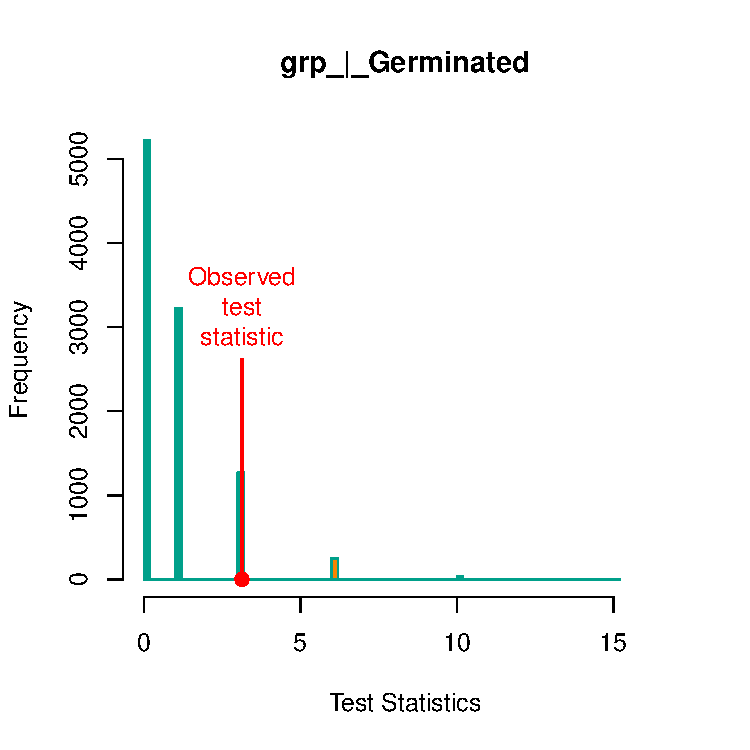
\includegraphics{LinearModel_booklet_files/figure-latex/unnamed-chunk-27-1} \end{center}

\hypertarget{analysis-of-variance}{%
\subsection{Analysis of variance}\label{analysis-of-variance}}

The Deviance Explained and (and\(R ^ 2\)) increases - does not decrease
- with each addition of variables (+ variables = + flexibility = better
fit). (warning: better fit doesn't correspond to a better generalization
to new data)

REMARK: this mean that we are considering \textbf{nested models}

for example:

\begin{Shaded}
\begin{Highlighting}[]
\KeywordTok{summary}\NormalTok{ (modelFull)}
\end{Highlighting}
\end{Shaded}

\begin{verbatim}
## 
## Call:
## lm(formula = Reaction.Time ~ Age + Gender + Age:Gender, data = reaction)
## 
## Residuals:
##     Min      1Q  Median      3Q     Max 
## -3.8859 -2.1954 -0.1279  1.5675  5.2472 
## 
## Coefficients:
##              Estimate Std. Error t value Pr(>|t|)  
## (Intercept)  18.73568    5.13680   3.647   0.0107 *
## Age           0.09812    0.09378   1.046   0.3358  
## GenderM     -12.34255    6.48970  -1.902   0.1059  
## Age:GenderM   0.13353    0.12480   1.070   0.3258  
## ---
## Signif. codes:  0 '***' 0.001 '**' 0.01 '*' 0.05 '.' 0.1 ' ' 1
## 
## Residual standard error: 3.608 on 6 degrees of freedom
## Multiple R-squared:  0.7611, Adjusted R-squared:  0.6416 
## F-statistic:  6.37 on 3 and 6 DF,  p-value: 0.02703
\end{verbatim}

\begin{Shaded}
\begin{Highlighting}[]
\NormalTok{modelAgeGen =}\StringTok{ }\KeywordTok{lm}\NormalTok{ (Reaction.Time }\OperatorTok{~}\StringTok{ }\NormalTok{Age }\OperatorTok{+}\StringTok{ }\NormalTok{Gender, }\DataTypeTok{data =}\NormalTok{ reaction)}
\KeywordTok{summary}\NormalTok{ (modelAgeGen)}
\end{Highlighting}
\end{Shaded}

\begin{verbatim}
## 
## Call:
## lm(formula = Reaction.Time ~ Age + Gender, data = reaction)
## 
## Residuals:
##     Min      1Q  Median      3Q     Max 
## -3.5372 -2.8513 -0.8364  3.1623  4.4334 
## 
## Coefficients:
##             Estimate Std. Error t value Pr(>|t|)   
## (Intercept) 14.81447    3.63652   4.074  0.00473 **
## Age          0.17353    0.06251   2.776  0.02746 * 
## GenderM     -5.86376    2.35899  -2.486  0.04186 * 
## ---
## Signif. codes:  0 '***' 0.001 '**' 0.01 '*' 0.05 '.' 0.1 ' ' 1
## 
## Residual standard error: 3.645 on 7 degrees of freedom
## Multiple R-squared:  0.7155, Adjusted R-squared:  0.6342 
## F-statistic: 8.801 on 2 and 7 DF,  p-value: 0.01229
\end{verbatim}

\begin{Shaded}
\begin{Highlighting}[]
\NormalTok{modelAge =}\StringTok{ }\KeywordTok{lm}\NormalTok{ (Reaction.Time }\OperatorTok{~}\StringTok{ }\NormalTok{Age, }\DataTypeTok{data =}\NormalTok{ reaction)}
\KeywordTok{summary}\NormalTok{ (modelAge)}
\end{Highlighting}
\end{Shaded}

\begin{verbatim}
## 
## Call:
## lm(formula = Reaction.Time ~ Age, data = reaction)
## 
## Residuals:
##    Min     1Q Median     3Q    Max 
## -6.535 -3.364 -0.272  2.676  7.839 
## 
## Coefficients:
##             Estimate Std. Error t value Pr(>|t|)  
## (Intercept) 10.30135    4.04407   2.547   0.0343 *
## Age          0.20647    0.07841   2.633   0.0300 *
## ---
## Signif. codes:  0 '***' 0.001 '**' 0.01 '*' 0.05 '.' 0.1 ' ' 1
## 
## Residual standard error: 4.678 on 8 degrees of freedom
## Multiple R-squared:  0.4643, Adjusted R-squared:  0.3973 
## F-statistic: 6.934 on 1 and 8 DF,  p-value: 0.03003
\end{verbatim}

From the analysis it seems that the interaction and the Gender are not
predictive. We test this hypothesis through a comparison of nested
models

\begin{Shaded}
\begin{Highlighting}[]
\KeywordTok{anova}\NormalTok{ (modelAgeGen, modelFull)}
\end{Highlighting}
\end{Shaded}

\begin{verbatim}
## Analysis of Variance Table
## 
## Model 1: Reaction.Time ~ Age + Gender
## Model 2: Reaction.Time ~ Age + Gender + Age:Gender
##   Res.Df    RSS Df Sum of Sq      F Pr(>F)
## 1      7 93.008                           
## 2      6 78.105  1    14.903 1.1448 0.3258
\end{verbatim}

Among the multiple models with or without interaction there is no
significant difference in terms of the explained variance.

With ANOVA test we make the following question: ``Does the exclusion of
predictor \(X\) decreases the predictability of the response?''. This
evaluation is not only based on the reduction of Residual Standard Error
(i.e.~decrease of Multiple R-squared), but also the reducted flexiblity
of the model (i.e.~the DF spent to model the tested variable \(X\)).

As index, the Adjusted R-squared is a more ``honest'' index of explained
variance then the Multiple R-squared.

Excluding the \(Gender\) variable instead does not seem like a good
idea:

\begin{Shaded}
\begin{Highlighting}[]
\KeywordTok{anova}\NormalTok{ (modelAge, modelAgeGen)}
\end{Highlighting}
\end{Shaded}

\begin{verbatim}
## Analysis of Variance Table
## 
## Model 1: Reaction.Time ~ Age
## Model 2: Reaction.Time ~ Age + Gender
##   Res.Df     RSS Df Sum of Sq      F  Pr(>F)  
## 1      8 175.104                              
## 2      7  93.008  1    82.096 6.1788 0.04186 *
## ---
## Signif. codes:  0 '***' 0.001 '**' 0.01 '*' 0.05 '.' 0.1 ' ' 1
\end{verbatim}

\ldots{} and not even removing \(Age\):

\begin{Shaded}
\begin{Highlighting}[]
\KeywordTok{anova}\NormalTok{ (modelGender, modelAgeGen)}
\end{Highlighting}
\end{Shaded}

\begin{verbatim}
## Analysis of Variance Table
## 
## Model 1: Reaction.Time ~ Gender
## Model 2: Reaction.Time ~ Age + Gender
##   Res.Df     RSS Df Sum of Sq      F  Pr(>F)  
## 1      8 195.390                              
## 2      7  93.008  1    102.38 7.7056 0.02746 *
## ---
## Signif. codes:  0 '***' 0.001 '**' 0.01 '*' 0.05 '.' 0.1 ' ' 1
\end{verbatim}

The best (most parsimonious) model is the one with
only\(Age\)and\(Gender\)but without interaction.

\hypertarget{model-selection-via-aic-and-bic}{%
\subsection{Model selection via AIC and
BIC}\label{model-selection-via-aic-and-bic}}

These are methods that penalize models with many predictors.

We compare the BIC (Bayesian Information Criterion) or the AIC (Akaike
Information Criterion) of the models. The idea: the lower the BIC and
the better the model

\begin{Shaded}
\begin{Highlighting}[]
\NormalTok{n =}\StringTok{ }\KeywordTok{nrow}\NormalTok{ (reaction)}
\NormalTok{(}\DataTypeTok{BIC1 =} \KeywordTok{AIC}\NormalTok{ (modelFull, }\DataTypeTok{k =} \KeywordTok{log}\NormalTok{ (n)))}
\end{Highlighting}
\end{Shaded}

\begin{verbatim}
## [1] 60.44635
\end{verbatim}

\begin{Shaded}
\begin{Highlighting}[]
\NormalTok{(}\DataTypeTok{BIC2 =} \KeywordTok{AIC}\NormalTok{ (modelAgeGen, }\DataTypeTok{k =} \KeywordTok{log}\NormalTok{ (n)))}
\end{Highlighting}
\end{Shaded}

\begin{verbatim}
## [1] 59.89008
\end{verbatim}

\begin{Shaded}
\begin{Highlighting}[]
\NormalTok{(}\DataTypeTok{BIC3 =} \KeywordTok{AIC}\NormalTok{ (modelAge, }\DataTypeTok{k =} \KeywordTok{log}\NormalTok{ (n)))}
\end{Highlighting}
\end{Shaded}

\begin{verbatim}
## [1] 63.91446
\end{verbatim}

\begin{Shaded}
\begin{Highlighting}[]
\NormalTok{(}\DataTypeTok{BICGender =} \KeywordTok{AIC}\NormalTok{ (modelGender, }\DataTypeTok{k =} \KeywordTok{log}\NormalTok{ (n)))}
\end{Highlighting}
\end{Shaded}

\begin{verbatim}
## [1] 65.01065
\end{verbatim}

(Also in this case) The model with \texttt{Age\ +\ Gender} seems to be
the best.

\begin{Shaded}
\begin{Highlighting}[]
\KeywordTok{summary}\NormalTok{ (modelAgeGen)}
\end{Highlighting}
\end{Shaded}

\begin{verbatim}
## 
## Call:
## lm(formula = Reaction.Time ~ Age + Gender, data = reaction)
## 
## Residuals:
##     Min      1Q  Median      3Q     Max 
## -3.5372 -2.8513 -0.8364  3.1623  4.4334 
## 
## Coefficients:
##             Estimate Std. Error t value Pr(>|t|)   
## (Intercept) 14.81447    3.63652   4.074  0.00473 **
## Age          0.17353    0.06251   2.776  0.02746 * 
## GenderM     -5.86376    2.35899  -2.486  0.04186 * 
## ---
## Signif. codes:  0 '***' 0.001 '**' 0.01 '*' 0.05 '.' 0.1 ' ' 1
## 
## Residual standard error: 3.645 on 7 degrees of freedom
## Multiple R-squared:  0.7155, Adjusted R-squared:  0.6342 
## F-statistic: 8.801 on 2 and 7 DF,  p-value: 0.01229
\end{verbatim}

\begin{Shaded}
\begin{Highlighting}[]
\NormalTok{eff <-}\StringTok{ }\KeywordTok{allEffects}\NormalTok{(modelAgeGen) }
\KeywordTok{par}\NormalTok{(}\DataTypeTok{mfrow=}\KeywordTok{c}\NormalTok{(}\DecValTok{1}\NormalTok{,}\DecValTok{2}\NormalTok{))}
\KeywordTok{plot}\NormalTok{(eff,}\StringTok{'Age'}\NormalTok{,}\DataTypeTok{ask=}\NormalTok{F,}\DataTypeTok{main=}\StringTok{'Age'}\NormalTok{) }
\end{Highlighting}
\end{Shaded}

\begin{center}\includegraphics{LinearModel_booklet_files/figure-latex/unnamed-chunk-34-1} \end{center}

\begin{Shaded}
\begin{Highlighting}[]
\KeywordTok{plot}\NormalTok{(eff,}\StringTok{'Gender'}\NormalTok{,}\DataTypeTok{ask=}\NormalTok{F,}\DataTypeTok{main=}\StringTok{'Gender'}\NormalTok{) }
\end{Highlighting}
\end{Shaded}

\begin{center}\includegraphics{LinearModel_booklet_files/figure-latex/unnamed-chunk-34-2} \end{center}

\begin{Shaded}
\begin{Highlighting}[]
\KeywordTok{par}\NormalTok{(}\DataTypeTok{mfrow=}\KeywordTok{c}\NormalTok{(}\DecValTok{1}\NormalTok{,}\DecValTok{1}\NormalTok{))}
\end{Highlighting}
\end{Shaded}

\end{document}
